\PassOptionsToPackage{unicode}{hyperref}
\documentclass[aspectratio=1610, 9pt]{beamer}

% Load packages you need here
\usepackage{polyglossia}
\setmainlanguage{english}

\usepackage{csquotes}
    

\usepackage{amsmath}
\usepackage{amssymb}
\usepackage{mathtools}

\usepackage{hyperref}
\usepackage{bookmark}
\usepackage[
  locale=UK,
  separate-uncertainty=true,
  per-mode=symbol-or-fraction,
]{siunitx}
\usepackage[
  backend=biber,   % use modern biber backend
  autolang=hyphen, % load hyphenation rules for if language of bibentry is not
  % german, has to be loaded with \setotherlanguages
  % in the references.bib use langid={en} for english sources
  sorting=none,
  ]{biblatex}
  \addbibresource{references.bib}  % the bib file to use
  \DefineBibliographyStrings{english}{andothers = {{et\,al\adddot}}}  % replace u.a. with et al.
  
  
% load the theme after all packages
\usetheme[
  showtotalframes, % show total number of frames in the footline
]{tudo}

% Put settings here, like
\unimathsetup{
  math-style=ISO,
  bold-style=ISO,
  nabla=upright,
  partial=upright,
  mathrm=sym,
}
\setbeamertemplate{caption}{\raggedright\insertcaption\par}

\title{Determining the dielectric function through THz-Transmission measurments}
\author[M.~Koch]{Max Koch}
\institute[AG Wang]{Arbeitsgruppe Wang \\  Fakultät Physik}
%\titlegraphic{\includegraphics[width=0.3\textwidth, angle=90]{images/setup.jpeg}}


\begin{document}

\maketitle

\section{Goal}
\begin{frame}
The First goal is to determine the refractive index 
\begin{equation}
  n_s = n - i\kappa
\end{equation}
which contains the real part $n$ and complex part $\kappa$ of the refractive index.
\end{frame}

\section{Scheme}
\begin{frame}{Scheme}
  Lets first take a look at the experimental scheme
  \begin{center}
  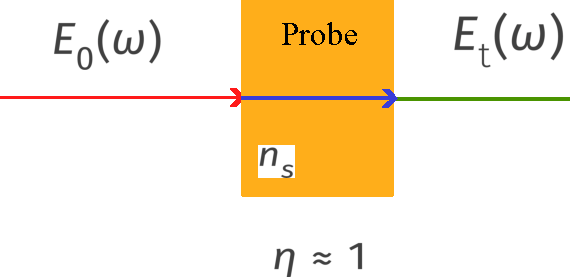
\includegraphics[width=0.5\textwidth]{images/Transmission.pdf}
  \end{center}
  The incoming THz-pulse $E_0(\omega)$ gets diffracted two times, indicated by the arrows, before it leaves the probe as the transmitted wave $E_\text{t}(\omega)$.
  For simplicity sake it is easier to assume an incident angel of $\theta=\SI{0}{\degree}$.
  All reflections are neglected.
  As defined earlier the probe has the refractive index $n_s$, its length is set to be $l$.
  The refractive index of the surrounding medium is $\eta$ in case of air $\eta\approx 1$.
\end{frame}

\begin{frame}{Transmitted wave}
  The transmitted wave is defined as 
  \begin{equation}
    E_\text{t}(\omega) = t(\omega) E_0(\omega)
  \end{equation}
  where
  \begin{equation}
    t(\omega) = \tau \tau' \symup{exp}\left[- i n_s(\omega) \frac{\omega l }{c}\right]
  \end{equation}
  is the transmission coeffiecient.
  The transmission coeffiecient is derived from the fresnel equations.
  Basically the wave is defracted two times, once when entering the medium and one when leaving the medium hence $\tau$ and $\tau'$.
  The defraction also generates a phase difference, which is represented by the exponential function.
  The complex transmission coeffiecients 
  \begin{align}
    \tau = & \frac{2}{1 + n_s} \\
    \tau' = &  \frac{2 n_s}{1+ n_s} 
  \end{align}
  are dependent on the refractive index $n_s$.
\end{frame}

\begin{frame}
  Lets do a first summary of our assumptions so far:
  \begin{itemize}
    \item No reflections
    \item Incident angle of $\theta=\SI{0}{\degree}$
    \item The probe is completly homogenous
  \end{itemize}
  with those assumptions the transmitted wave can be written as 
  \begin{equation}
    E_\text{t}(\omega) = \eta\frac{4 n_s (\omega)}{(n_s(\omega) + 1)^2} \symup{exp}\left[ -i n_s (\omega) \frac{\omega l }{c}\right] E_0(\omega)
  \end{equation}
\end{frame}

\begin{frame}{References measurment}
  To determine the refractive index it is necessary to know the properties of the uninterrupted THz-pulse.
  For this a references measurment of the THz-pulse is taken.
  The references wave 
  \begin{equation}
  E_\text{ref}(\omega) = \eta \symup{exp}\left[ -i \frac{\omega l }{c}\right] E_0(\omega)  
  \end{equation}
  sligthly differs from the original THz-pulse $E_0(\omega)$ as it travels through the space of length $l$, which was filled by the probe medium prior.
  \begin{center}
  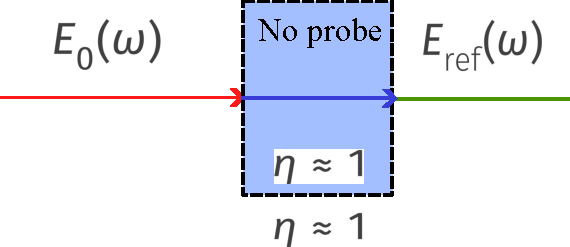
\includegraphics[width=0.5\textwidth]{images/reference.pdf}
  \end{center}
\end{frame}

\section{Complex transfer function}
\begin{frame}{Complex transfer function}
  With the transfered wave $E_\text{t}(\omega)$ and the reference wave $E_\text{ref}(\omega)$ a complex transfer function 
  \begin{equation}
    H_0(\omega) = \frac{E_\text{t}(\omega)}{E_\text{ref}(\omega)}
  \end{equation}
  can be defined.
  After plugging in the definitions of $E_\text{t}(\omega)$ and $E_\text{ref}(\omega)$, $H_0(\omega)$ yields
  \begin{equation}
    H_0 (\omega) = \frac{4 n_s(\omega)}{(n_s(\omega) +1)^2} \symup{exp}\left[-\kappa(\omega) \frac{\omega l }{c}\right] \symup{exp}\left[-i (n (\omega) - 1) \frac{\omega l}{c}\right]
  \end{equation}
  \end{frame}

\begin{frame}{Extracting phase}
  As the complex refractive index inside the exponent of $H_0(\omega)$ is rather tricky to solve it is assumed that the complex refractive index is similar to its real part $n_s(\omega) \approx n(\omega)$.
  This simplifies to 
  \begin{equation}
    H(\omega) = \frac{4n(\omega)}{(n(\omega) + 1)^2} \symup{exp}\left[-\kappa(\omega) \frac{\omega l }{c}\right] \symup{exp}\left[- i(n(\omega) - 1) \frac{\omega l}{c}\right]
  \end{equation}
  of which the phase information is
  \begin{equation}
    \Phi(H(\omega)) = -[n(\omega) - 1] \frac{\omega l}{c}
  \end{equation}
  and the logarithm is
  \begin{equation}
    \symup{ln}|H(\omega)| = \symup{ln}\left[ \frac{4n(\omega)}{(n(\omega) +1)^2}\right] - \kappa(\omega) \frac{\omega l}{c} \, .
  \end{equation}
\end{frame}

\begin{frame}{Determining the refractive index}
  With the phase information and logarithm it is now possible to determine the real refractive index 
  \begin{equation}
    n(\omega) = 1 - \frac{c}{\omega l} \Phi(H(\omega))
  \end{equation}
  and the complex refractive index 
  \begin{equation}
    \kappa(\omega) = \frac{c}{\omega l } \left( \symup{ln}\left[ \frac{4 n(\omega)}{(n(\omega) + 1)^2}\right] - \symup{ln}|H(\omega)|\right)
  \end{equation}
  from which the absorption coeffiecient
  \begin{equation}
    \alpha(\omega) = \frac{2 \omega \kappa(\omega)}{c}
  \end{equation}
  can be calculated.
  Note that a special unwrapping process is necessary to determine $\Phi(H(\omega))$, in python \textit{numpy.unwrap()} can be used to do this.
\end{frame}

\begin{frame}{Example data}
  By using the discussed methods a reference dataset is analyzed.
  The measured data is plotted below 
  \begin{center}
    \begin{columns}
      \begin{column}{0.5\textwidth}
        \begin{figure}
          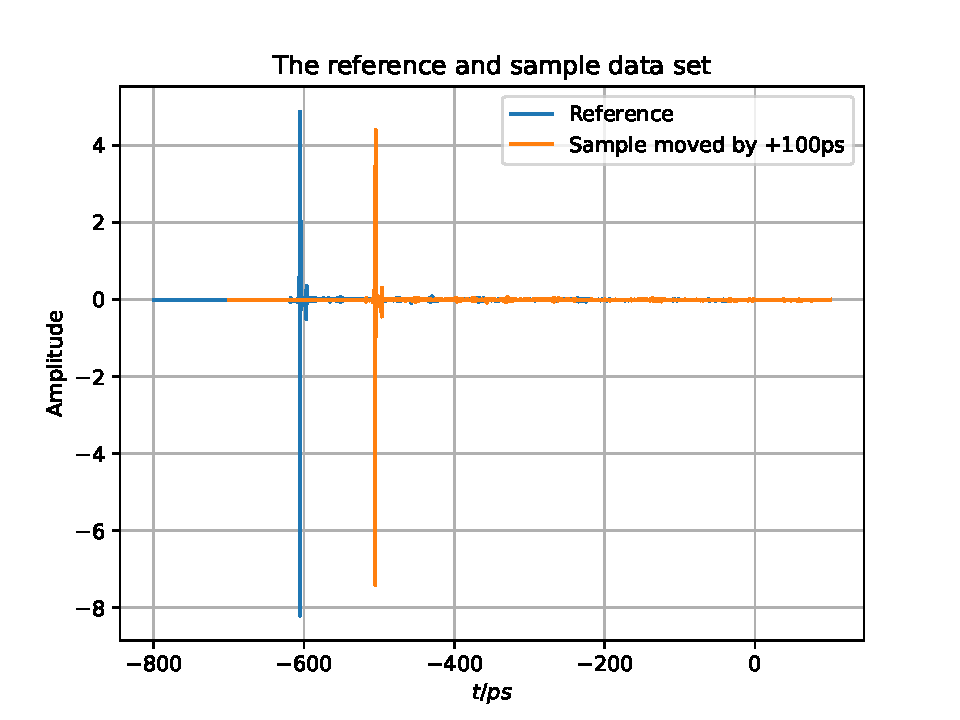
\includegraphics[width=0.8\textwidth]{images/THz1.pdf}
          \caption{Some transmission data of Teflon foil, with a thickness of $\SI{0.25}{\milli\meter}$.}
        \end{figure}
      \end{column}
      \begin{column}{0.5\textwidth}
        \begin{figure}
          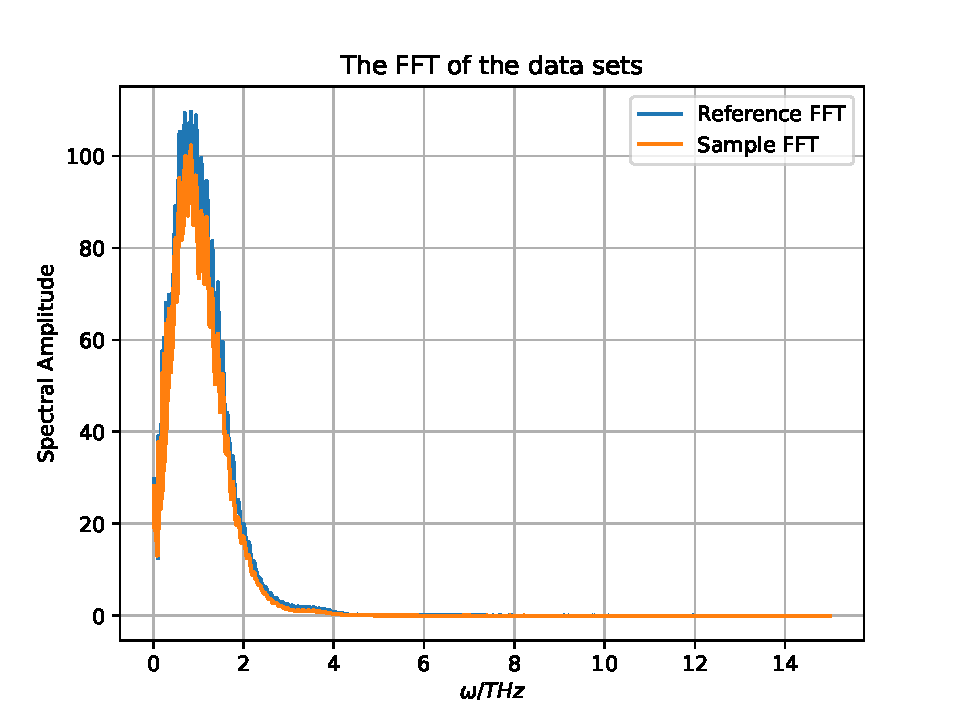
\includegraphics[width=0.8\textwidth]{images/THz4_1.pdf}
          \caption{The FFT of the transmission data of Teflon foil, with a thickness of $\SI{0.25}{\milli\meter}$.}
        \end{figure}
      \end{column}
    \end{columns}
  \end{center}
\end{frame}

\begin{frame}{Refractive index}
  The refractive index is then determined by the Quotient of Transmission and reference data in frequency space.
  \begin{equation}
    n(\omega) = 1 - \frac{c}{\omega l} \Phi(H(\omega))
  \end{equation}
  The result can be seen below:
  \begin{center}
    \begin{figure}
      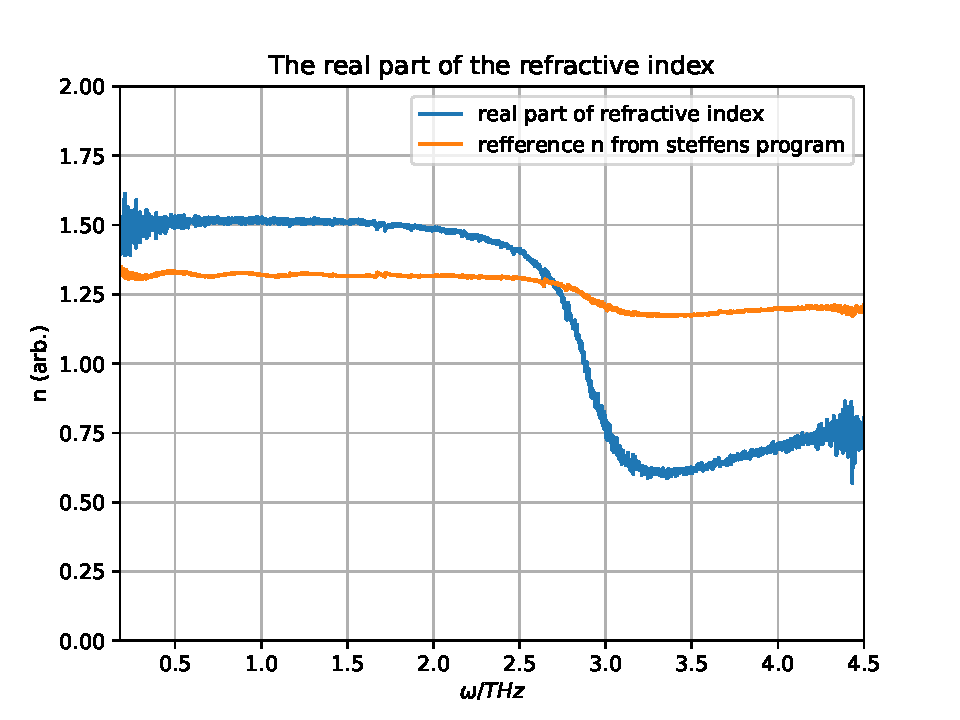
\includegraphics[width=0.5\textwidth]{images/THz5_1.pdf}
      \caption{The refractive index of Teflon as calculated by the equation shown above.}
    \end{figure}
  \end{center}
\end{frame}

\begin{frame}{Absorption coeffiecient}
  The absorption coeffiecient is then determined by
  \begin{equation}
    \alpha(\omega) = \frac{2 \omega \kappa(\omega)}{c}
  \end{equation}
  where $\kappa$ is the complex refractive index, which is determined by 
  \begin{equation}
    \kappa(\omega) = \frac{c}{\omega l } \left( \symup{ln}\left[ \frac{4 n(\omega)}{(n(\omega) + 1)^2}\right] - \symup{ln}|H(\omega)|\right)
  \end{equation}
  The result can be seen below:
  \begin{center}
    \begin{figure}
      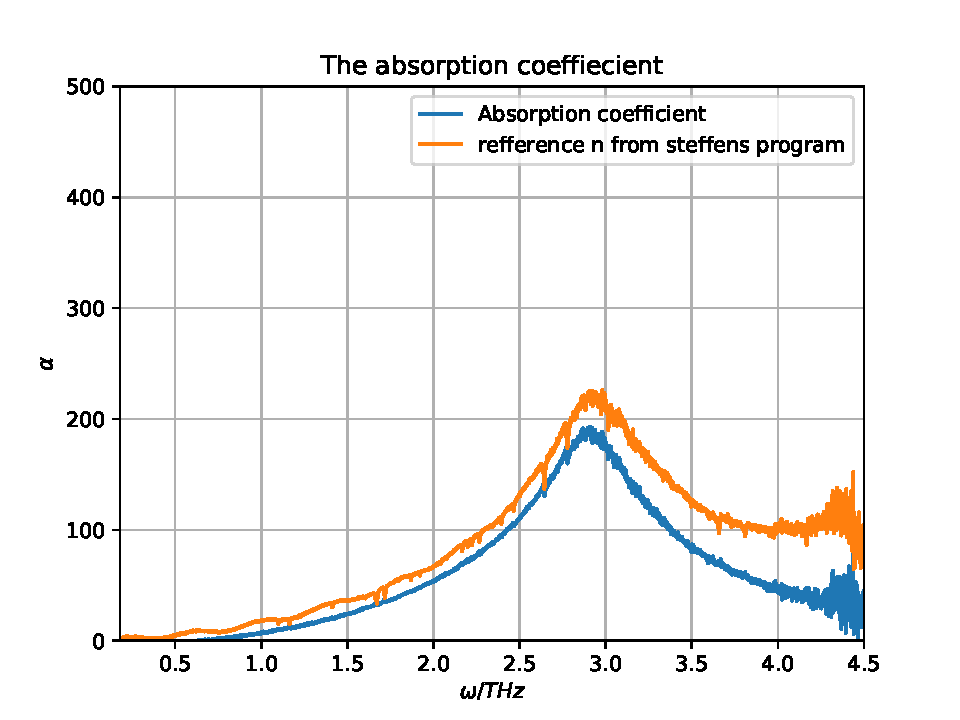
\includegraphics[width=0.4\textwidth]{images/THz6.pdf}
      \caption{The absorption coeffiecient of Teflon as calculated by the equation shown above.}
    \end{figure}
  \end{center}
\end{frame}

\begin{frame}{Phase}
  Just as a reference we can also plot the phase information that we derive from the time resolved measurment.
  The result can be seen below:
  \begin{center}
    \begin{figure}
      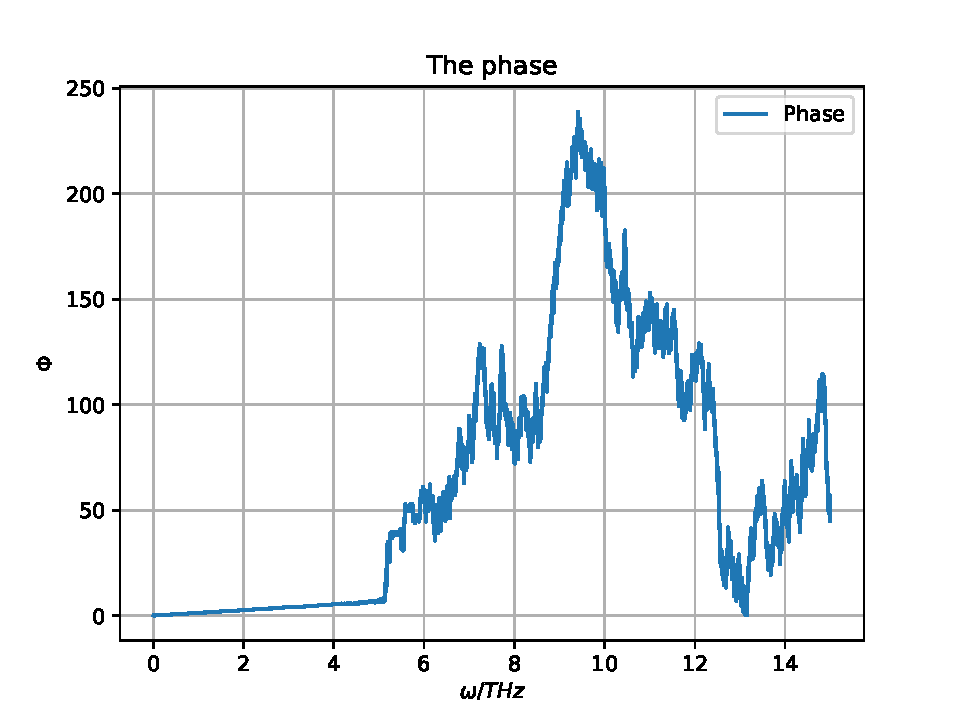
\includegraphics[width=0.5\textwidth]{images/THzPhase.pdf}
      \caption{The Phase of Teflon as calculated by the equation shown above.}
    \end{figure}
  \end{center}
  As you can see in this Example the Phase and angle of the Transferfunction $H_0$ align.
  This is because the angle does not extend over $2\pi$.
\end{frame}


\begin{frame}{Fabry-Perot factor}
  Now lets take a look at the reflections inside the probe.
  The fresnel equations tell us that for every additional path that the wave takes inside the medium we have to multiply it by 
  \begin{equation}
    \rho'^2 = \left(\frac{1 - n_s}{1 + n_s}\right)^2
  \end{equation}
  aswell as a phase shift factor 
  \begin{equation}
    \Phi = \symup{exp}\left[-k \cdot i n_s \frac{\omega l}{c}\right]
  \end{equation}
  where $k$ is the number transmissions inside the probe.
  \begin{figure}
    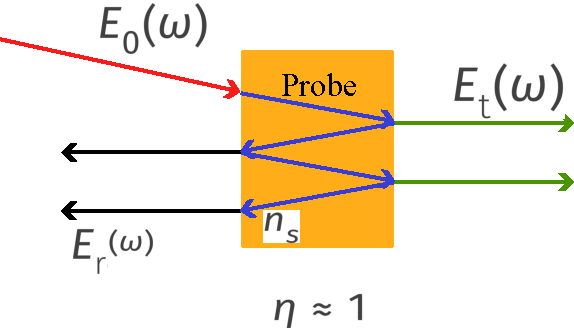
\includegraphics[width=0.4\textwidth]{images/Perot.pdf}
    \caption{Through reflections inside the medium the transmitted wave $E_\text{t}(\omega)$ will consist of several phase shifted reflections.}
  \end{figure}
\end{frame}

\begin{frame}
  If we consider all the reflections inside the probe the transmitted wave will look like
  \begin{align*}
    E_\text{t}(\omega) \,=\,& \tau \tau' \symup{exp} \left[-i n_s(\omega) \frac{\omega l }{c}\right] \\
                        & \cdot \left( 1 + \rho'^2 \cdot \symup(exp)\left[ -3 i n_s(\omega) \frac{\omega l }{c}\right] + \rho'^4 \symup(exp) \left[ -5 i n_s(\omega) \frac{\omega l }{c}\right] + ...\right) \cdot E_0 (\omega) \\
                        \,=\,& \tau \tau' \symup(exp)\left[ -2 i n_s(\omega) \frac{\omega l }{c}\right] \cdot FP(\omega) E_0(\omega)
  \end{align*}
  where $\rho'$ is the complex reflection coeffiecient of the probe
  \begin{equation}
    \rho' = \frac{1 - n_s}{1 + n_s}
  \end{equation}
  and $FP(\omega)$ is the Fabry-Perot Factor, which can be expressed as 
  \begin{equation}
    FP(\omega) = \left[1 - \rho'^2 \cdot \symup(exp)\left(- 2 i n_s(\omega )\frac{\omega l }{c}\right)\right]^{-1}
  \end{equation}
\end{frame}

\begin{frame}{2D-Materials}
  The last "challenge" is to estimate the refractive index of very thin materials.
  Spectroscopy setups are usually achieved by using a substrate on which the 2D-material will be applied.
  The result is a signal from the substrate and a very weak signal from the 2D-material.
  \begin{figure}
    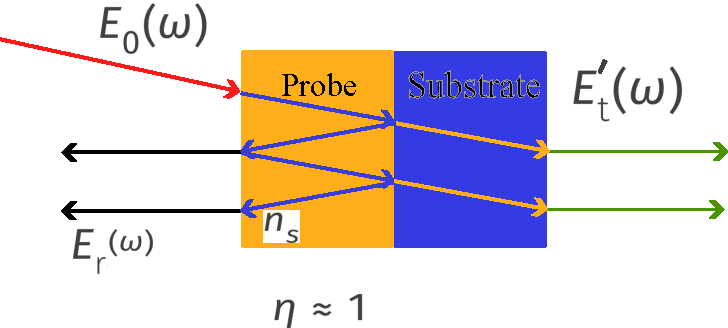
\includegraphics[width=0.5\textwidth]{images/2d.pdf}
    \caption{The Probe is applied onto a substrate that also alters the intial THz-wave.}
  \end{figure}
\end{frame}

\begin{frame}
  For this we have to consider the transmission coeffiecients $t(\omega)$ of both mediums.
  Aswell as reflections inside the medium.
  We can write the transmitted THz-wave as
  \begin{equation}
    E_\text{t} '(\omega) = \eta t_\text{Probe}(\omega) t_\text{Sub}(\omega)FP(\omega)E_0(\omega)
  \end{equation}
  where $t_\text{Probe}(\omega)$ and $t_\text{Sub}(\omega)$ denote the transmission coeffiecients of the probe and substrate respectively.
  The complex transfer function $H_0'$ can then be writen as 
  \begin{equation}
    H_0(\omega) = \frac{3 n_s \cdot n_\text{sub}}{(1 + n_s)(n_s + n_\text{sub})} \symup{exp}\left[-i (n_s - 1)\frac{\omega l}{c}\right]FP(\omega)
  \end{equation}
  \textcolor{red}{hier bin ich nicht ganz sicher mit den faktoren}
\end{frame}

\section{conclusion}
\begin{frame}{Refractive index}
  The refractive index can now be calculated by the formula defined in the beginning
  \begin{equation}
    n_s(\omega) = n - i \kappa \, .
  \end{equation}
  \newline
  \textcolor{tugreen}{conclusion:} This scheme gives an easy way to determine the refractive index of thick homogenous probes through time resolved THz-Spectroscopy.
  It can be extended to also take reflections inside the probe into account by using the Fabry-Perot factor in the transmitted wave.
  However, for most experimental setups this wont be necessary as the post-pulse is sufficiently delayed.

\end{frame}
\end{document} 